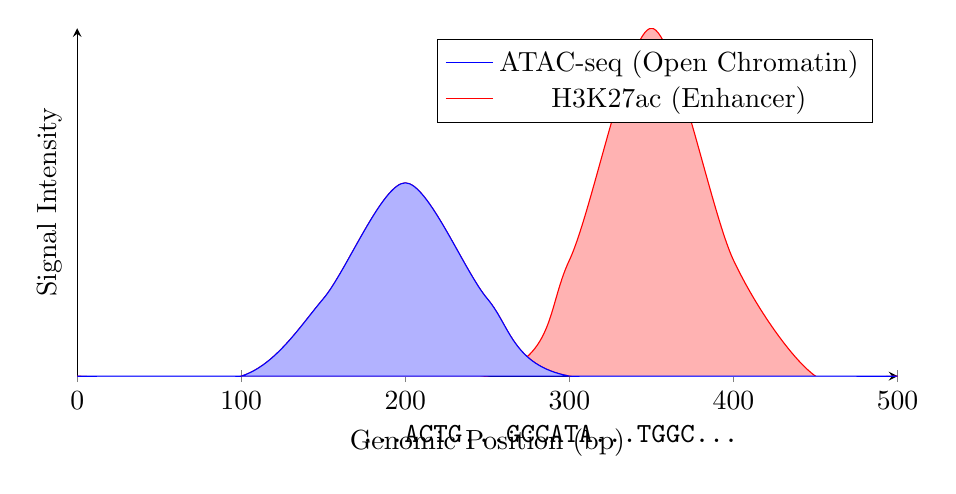
\begin{tikzpicture}
\begin{axis}[
    width=12cm, height=6cm,
    axis x line=bottom,
    axis y line=left,
    ylabel={Signal Intensity},
    xlabel={Genomic Position (bp)},
    ytick=\empty,
    xtick={0, 100, 200, 300, 400, 500},
    legend pos=north east,
    stack plots=y
]

% ATAC-seq Peak
\addplot[fill=blue!30, draw=blue, smooth] coordinates {
    (0,0) (100,0) (150,10) (200,25) (250,10) (300,0) (500,0)
} \closedcycle;
\addlegendentry{ATAC-seq (Open Chromatin)}

% ChIP-seq Peak (Shifted)
\addplot[fill=red!30, draw=red, smooth] coordinates {
    (0,0) (250,0) (300,5) (350,20) (400,5) (450,0) (500,0)
} \closedcycle;
\addlegendentry{H3K27ac (Enhancer)}

\end{axis}
% Sequence context annotation
\node[anchor=north] at (6,-0.5) {\texttt{...ACTG...GCCATA...TGGC...}};
\end{tikzpicture}
